% ===================================================================================================
%                                                 |                                                 |
%                                                 |                                                 |
% -------------------------------------------- SECTION ---------------------------------------------|
%                                                 |                                                 |
%                                                 |                                                 |
% ===================================================================================================
\section{Introduction}\label{sec:intro}
%---
\begin{fancyquotes}
	AI is one of the cornerstones of the growing digitization of industry ('Industry 4.0'). Technologies underpinning  this  process  ---  such as IoT,  5G,  \textbf{cloud  computing},  big  data  analytics,  \textbf{smart  sensors},  augmented  reality,  3D  printing  and  \textbf{robotics}  ---  are  likely  to  transform  manufacturing  into  a  single cyber-physical  system  in which digital  technology,  internet  and  production  are merged in one \cite{szczepanski_2019}.
\end{fancyquotes}
%---
\textcolor{red}{As technology develops, not only smart factories will become the norm, but healthcare services modernize and household evolve into mostly automated environments. Modern industrial, cooperative, service, and healthcare robots with local and network computing capabilities would populate all these environment, collecting and sharing data from their various sensors.} AI will be a natural component of these robots, enabling them to learn new skills and spread their acquired knowledge across systems. The more these \emph{embodied AI} (EIA) agents integrate synergistically into manufacturing, the more they will take over diverse tasks while also actively cooperating with humans. Yet, as EAI agents become ubiquitous, new challenges will emerge, among them, their energy demands.

% SUBSECTION ========================================================================================
\subsection{The energy problem in classical and embodied AI}
%---
% \begin{figure}[!t]
% 	\centering
% 	\includegraphics[width=0.99\columnwidth]{fig/smart_factory.pdf}
% 	\caption{The smart factory.}
% 	\label{fig:smartFactory}
% \end{figure}

Classical AI interprets intelligence as a purely computational symbol-processing problem decoupled from physical agents. Progress in classical AI relies on two computing stages: (i) learning and (ii) deployment. While the latter is not energy-efficient compared to its biological counterparts, the former craves a large energy quota to process large amounts of data for training, validation, and testing of models (e.g., supercomputing). Furthermore, both model and training data are expected to carry enough information to transfer knowledge between different tasks and even systems (at least to a certain extent). However, retraining is required when this information is unavailable in the data ---sometimes even from scratch---, leading to highly energy-inefficient learning paradigms. The implication is that the energetic cost of classical AI can sometimes outweigh the benefits \cite{Strubell2019EnergyAP}.

With the evolution towards embodied AI systems, i.e., the emerging field between AI and robotics, the challenges mentioned before expand. Since the real world cannot be faithfully replicated in virtual environments, and in spite the considerable advances in sim-to-real applications \cite{Chebotar2019Closingsimreal}, data acquisition in EAI agents necessitates constant and active energy-expending interaction with the physical environment. Likewise, in the real world, learning a skill implies physically executing it, and with each execution, energy is required for motion and interaction. Consider autonomous driving, where the vehicle is a rather rudimentary form of an EAI agent. Despite operating primarily in a structured human-made environment, complexity is already present in the system, as the vehicle spends energy simply by carrying out its purpose: autonomous movement; but also spends energy by collecting vast amounts of data (obtained by driving around) to retrain and improve the policy model. \textcolor{red}{Household robots are another example, current estimates indicate that 39\% of the domestic chores could be automated in the short term \cite{Lehdonvirta2022futuresunpaidwork}. Yet, even when compared to factory floors, homes still represent challenging dynamic environments that require EAI agents to undergo constant retraining.} While the energy demand of AI and robotics entered the scope of separate research communities in the last few years, the study of the energetic requirements of embodied AI and its vast implications has not received proper attention. 
% ---
\begin{figure*}[!t]
	\centering
	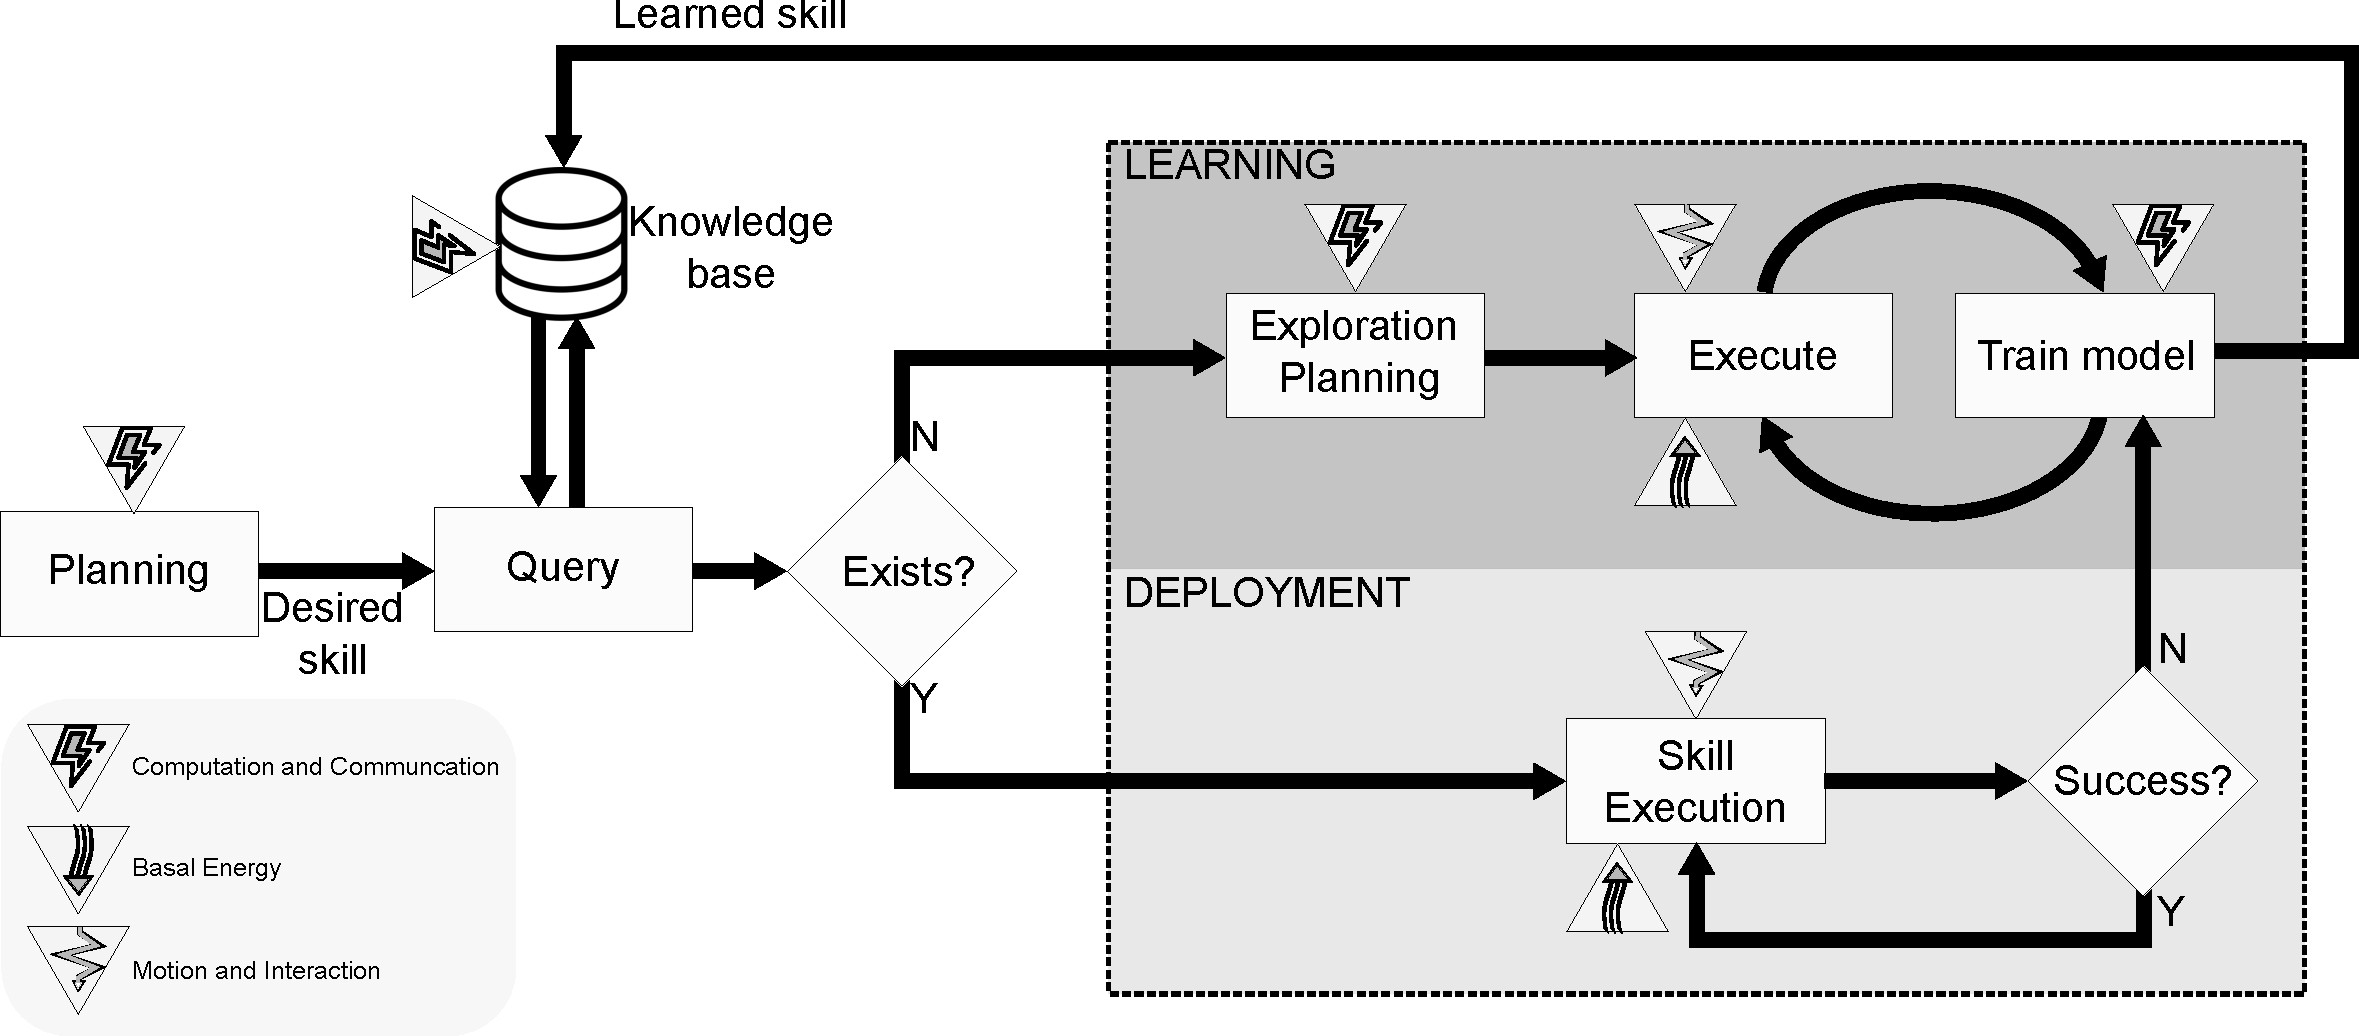
\includegraphics[width=0.9\textwidth]{fig/embodied_ai_learning_pipeline_v7.pdf}
	\caption{Standard skill execution pipeline of isolated EAI agents.}
	\label{fig:embodied_ai_pipeline}
\end{figure*}
% ---
% SUBSECTION ========================================================================================
\subsection{Contributions}
To facilitate the study of the energetic demand of EAI agents, we look at the standard skill execution pipeline from an isolated agent, shown in Fig.~\ref{fig:embodied_ai_pipeline}, and identify three main categories of energy usage, namely
% ---
\begin{enumerate}
	\item Computation and Communication Expenditure (CCE): Refers to the energy required by the computation process itself (e.g., the number of floating point operations) and by the supporting communication processes
	\item Basal Energy Expenditure (BEE): This is the energy associated with the basic functions of the EAI agent. For example, gravity compensation and proprioceptive intelligence/algorithms in robots, hovering in drones, collision avoidance in autonomous vehicles, etc.
	\item Motion and Interaction Expenditure (MIE): Defines the energy spent on executing a particular skill in a certain form
\end{enumerate}
% ---
Consequently, we provide projections on the growing energetic challenges in embodied AI pertaining to these categories and show that the energy demand scales out of proportion with the number of EAI agents if learning paradigms that do not promote and systematically exploit knowledge exchange persist. Furthermore, we establish that with the scaling complexity of the problems faced by classical and embodied AI, clever learning methods are required that not only make efficient use of the computation and physical power of the embodied agent but also leverage modern communication infrastructure to optimally collect, share, and transfer the knowledge acquired by other agents performing similar skills. For this, we contextualize the problem in a hypothetical case study using empirical/reported energy consumption estimations and introduce a full energy estimation model that accounts for the three energy expenditure categories (CCE, BEE, and MIE). Concretely, we estimate the substantial effect that our recently introduced paradigm of \emph{collective learning} can have on energy and time saving components in a smart factory scenario with many robots performing many skills. We show that collective learning is the natural solution to address the energy problem in embodied AI.

% SUBSECTION ========================================================================================
\subsection{Paper organization}
The remainder of this work is arranged as follows. In Sec.~\ref{sec:energy_demand_embodied_ai}, we discuss the energy demands brought about by the two main components of embodied AI: machine learning algorithms and robotics. Consequently, in Sec.~\ref{sec:energy_grand_challenges}, three grand challenges accompanying EAI systems in the context of their energy consumption are introduced. A brief mathematical formulation of the energy and time requirements of four learning paradigms employed with EAI agents is presented in Sec.\ref{sec:learning_paradigms} and used in Sec.~\ref{sec_use_case} in a use-case related to a smart factory to contrast these requirements against each other. Finally, in Sec.~\ref{sec:conclusion}, we summarize the paper and provide conclusions regarding the importance of knowledge sharing and transfer among EAI agents. 